\documentclass[a4paper]{article}
\usepackage[utf8]{inputenc}
\usepackage{tabularx}
\usepackage{anysize}
\usepackage{amsmath}
\usepackage{amsthm}
\usepackage{amssymb}
\usepackage{amsfonts} 
\usepackage{enumerate}
\usepackage{enumitem}
\usepackage{multicol}
\usepackage{graphicx}
\usepackage{tabularx}
\usepackage{float}
\usepackage{cprotect}
\usepackage[italian]{babel}
\usepackage[
    colorlinks = true,
    linkcolor = black,
    urlcolor  = black,
    citecolor = blue,
    anchorcolor = blue
]{hyperref}

\marginsize{2cm}{2cm}{1cm}{1cm}
\setlength{\parindent}{0cm}

\title{
Formal Languages and Compilers \\
Project \\
roda Compiler
}
\author{
    19598 Roland Bernard \\
    19615 Daniel Planötscher
}
\date{\today}

\newcommand{\nonterm}[1]{\, \mathit{#1} \,}
\newenvironment{changemargin}[2]{%
\begin{list}{}{%
\setlength{\topsep}{0pt}%
\setlength{\leftmargin}{#1}%
\setlength{\topmargin}{#2}%
\setlength{\rightmargin}{#1}%
\setlength{\listparindent}{\parindent}%
\setlength{\itemindent}{\parindent}%
\setlength{\parsep}{\parskip}%
}%
\item[]}{\end{list}}

\begin{document}

\maketitle

\section{Introduzione}

Roda è un piccolo linguaggio di programmazione strongly typed e compilato che utilizza una syntax moderna.

Il linguaggio roda contiene le seguenti caratteristiche:
\begin{itemize}
    \item Funzioni (con supporto per la chiamata di funzioni variadiche)
    \item Condizionali con espressioni if-else
    \item Cicli while
    \item Puntatori
    \item Espressioni aritmetiche su numeri interi e a virgola mobile
    \item Operazioni binarie su numeri interi
    \item Espressioni booleane
    \item Array
    \item Inference di tipi
    \item Alias di tipi
\end{itemize}

Inoltre, il compilatore prova a dare messaggi di errore utili e informativi.

\section{Linguaggio}

Quello che segue è un semplice programma hello-world scritto in roda:
\begin{verbatim}
extern fn printf(fmt: *u8, ..);

pub fn main(): int {
    printf("Hello world!\n");
    return 0;
}
\end{verbatim}

L'esempio seguente mostra le strutture di controllo supportate e il loro utilizzo:
\begin{verbatim}
extern fn printf(fmt: *u8, ..);

pub fn main(): int {
    let i = 1;
    while i <= 100 {
        if i % 3 == 0 && i % 5 == 0 {
            printf("FizzBuzz\n");
        } else if i % 3 == 0 {
            printf("Fizz\n");
        } else if i % 5 == 0 {
            printf("Buzz\n");
        } else {
            printf("%li\n", i);
        }
        i += 1;
    }
    return 0;
}
\end{verbatim}

Le altre caratteristiche possono essere utilizzate nel modo seguente:
\begin{itemize}
\item Espressioni aritmetiche 
\begin{verbatim}
let x = 1 + 2;          // x = 3
x += 5;                 // x = 8
// x += 0.5;            // real literals can not be implicitly converted to integers
x += 0.5 as int;        // x = 8
let y: f64 = 0.5 + 0.1; // y = 0.6
// y += 5;              // integer literals can not be implicitly converted to floats
y += 5 as f64;          // y = 5.6
\end{verbatim}

\item Puntatori
\begin{verbatim}
let a = *b; // take the address of b and store it into a
let c = &a; // dereference a to store its value into c
&a = c;     // assign the value in c to the address pointed to by a
\end{verbatim}

\item Array
\begin{verbatim}
let a: [3]int; // create an array of 3 ints
a[0] = 1;      // assign the value 1 to the first element of a
a[1] = 2;      // assign the value 2 to the second element of a
a[2] = a[1];   // assign the value 3 to the third element of a
\end{verbatim}

\item Inference di tipi
\begin{verbatim}
let a = 1;                  // a is an integer
let b = 2.0;                // b is a floating point number
let c = "Hello";            // c is a string
let d = true;               // d is a boolean value
let e = 'a';                // e is a character
let f;
a += f;                     // f is also an integer
let g = [[1, 2], [3, 4]];   // g is of type [2][2]int;
\end{verbatim}

\item Alias di tipi
\begin{verbatim}
type MyInt = int;  // create a type alias for int
let a: MyInt = 1;  // a is an integer
\end{verbatim}
\end{itemize}

\begingroup
\catcode`\%=12
\begin{table}[H]
\begin{tabularx}{0.55\textwidth}{|X|l|}
\hline
\textbf{Operatori} & \textbf{Associatività} \\
\hline
Function calls, array indexing & \\
\hline
Unary \verb?+ - * ! &? & \\
\hline
\verb?as? & \\
\hline
\verb?* / %? & left to right \\
\hline
\verb?+ -? & left to right \\
\hline
\verb?<< >>? & left to right \\
\hline
\verb?&? & left to right \\
\hline
\verb?^? & left to right \\
\hline
\verb?|? & left to right \\
\hline
\verb?== != < > <= >=? & left to right \\
\hline
\verb?&&? & left to right \\
\hline
\verb?||? & left to right \\
\hline
\end{tabularx}
\end{table}
\endgroup
La tabella precedente mostra la precedenza degli operatori del linguaggio, con gli operatori a
precedenza più alta indicati in alto. 
La grammatica della lingua viene mostrata nell'ultima pagina ed è una grammatica ambigua che,
con l'uso delle precedenze di sopra, può essere resa non ambigua.


\section{Implementazione}

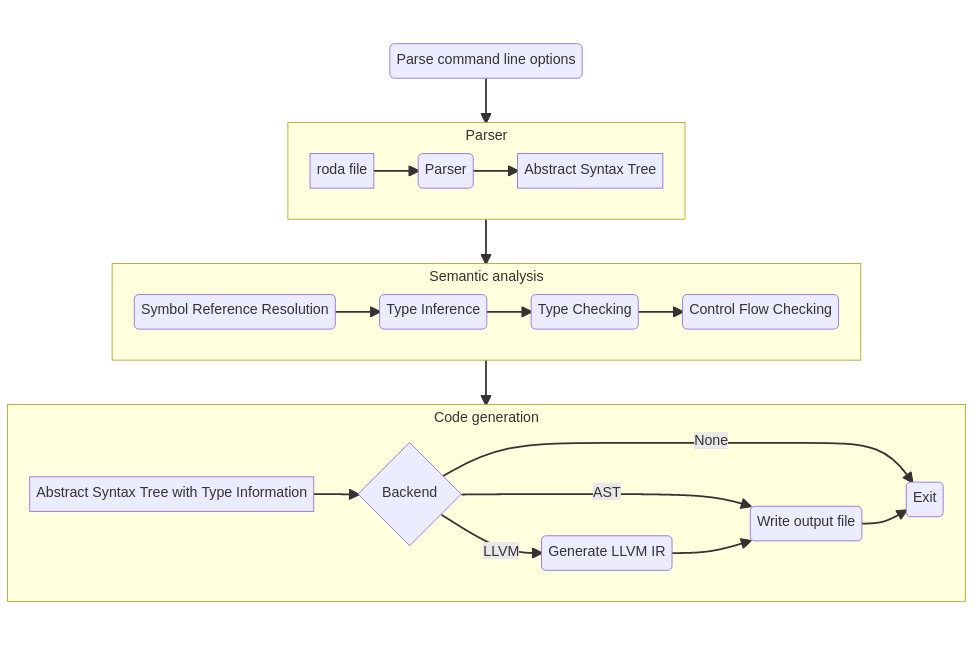
\includegraphics[width=\textwidth]{implementation.png}

Abbiamo scelto un'architettura di compilazione multi-pass, che opera principalmente su un abstract syntax tree.
Quello che segue sono i passaggi principali che compongono il processo di compilazione:

\begin{itemize}
    \item \textbf{Parser:}

    In questa fase, il compilatore legge il contenuto di un file e crea un abstract syntax tree utilizzando un lexer definito con Flex e un parser generato con Bison.

    \item \textbf{Symbol Reference resolution:}

    In questa fase, il compilatore risolve tutti i riferimenti ai simboli, sia per le variabili che
    per i tipi, nell'abstract syntax tree. Questa fase genera e utilizza anche le symbol tables,
    creando un'entry di simbolo per ogni tipo, funzione e variabile definita. Questa fase genera e
    utilizza anche le symbol tables, creando un'entry di simbolo per ogni tipo, funzione e variabile
    definita. La tabella dei simboli è implementata come un tree con solo parent-pointer. Ogni nodo
    dell'albero rappresenta uno scope, implementato con una hash table. La ricerca dei simboli inizia
    da un nodo e prosegue fino alla root, fino a quando trova il simbolo. I tipi e i simboli
    condividono la stessa hash table, ma sono gestiti in modo diverso.

    \item \textbf{Type Inference:}

    In questa fase, il compilatore infonde (infers) i tipi delle variabili e delle
    espressioni nell'abstract syntax tree. Questa
    fase risolve prima tutte le annotazioni di tipo esplicitamente fornite e i
    constraint impliciti di tipo (ad esempio, le nelle condizioni "if").
    Poi cerca d'inferire tutti gli altri tipi. L'inferenza dei tipi è
    implementata propagando i tipi usando l'attraversamento del grafo. Il
    compilatore inoltre, se il tipo non può essere altrimenti determinato,
    assume il tipo dei letterali interi e reali. Durante questa fase possono
    essere identificati e segnalati conflitti di tipo.

    \item \textbf{Type Checking:}

    In questa fase, il compilatore controlla che tutti i tipi dell'abstract syntax tree siano
    corretti. Questo comprende, ad esempio, l'uso di solo tipi numerici per l'addizione o la
    moltiplicazione, o il controllo del numero corretto di argomenti che venga passato a una
    chiamata di funzione. Inoltre, questa fase si assicura che il tipo di ogni variabile ed
    espressione sia stato dedotto con successo. Al termine di questa fase, l'abstract syntax tree
    è stato popolato con tipi validi.

    \item \textbf{Control Flow Checking:}
    
    In questa fase, il compilatore controlla che tutte le funzioni che dovrebbero restituire un
    valore, lo facciano effettivamente in ogni possibile branch attraverso il control-flow graph.
    Dopo questa fase, l'abstract syntax tree è garantito che rappresenti un programma valido, che
    può essere utilizzato per generazione di codice.

    \item \textbf{Code generation:}

    In questa fase, il compilatore genera il codice per l'abstract syntax tree. Questa fase può
    sempre non fare nulla o scrivere l'albero della sintassi astratta in un file. Può anche, se
    compilato con il supporto per questo, generare l'IR LLVM e usarlo per generare un file di
    assembly o di object. Opzionalmente, questa fase può includere anche un'invocazione del
    compilatore C del sistema per il linking.
\end{itemize}

\newpage

\begin{changemargin}{-1.5cm}{-2.5cm}
\begin{tabular}{lr}
$\cprotEnv\begin{aligned}
\nonterm{Program} \rightarrow& \, \nonterm{RootStatements}
\\
\nonterm{RootStatements} \rightarrow& \, \epsilon \\
    |& \, \nonterm{RootStatements} \nonterm{RootStatement} \\
    |& \, \nonterm{RootStatements} \, \verb?;? \,
\\
\nonterm{RootStatement} \rightarrow& \, \, \verb?pub? \, \, \verb?fn? \, \nonterm{Identifier} \, \verb?(? \, \nonterm{Parameters} \, \verb?)? \, \nonterm{OptionalType} \nonterm{Block} \\
    |& \, \, \verb?extern? \, \, \verb?fn? \, \nonterm{Identifier} \, \verb?(? \, \nonterm{Parameters} \, \verb?)? \, \nonterm{OptionalType} \, \verb?;? \, \\
    |& \, \, \verb?fn? \, \nonterm{Identifier} \, \verb?(? \, \nonterm{Parameters} \, \verb?)? \, \nonterm{OptionalType} \nonterm{Block} \\
    |& \, \, \verb?type? \, \nonterm{Identifier} \, \verb?=? \, \nonterm{Type} \, \verb?;? \,
\\
\nonterm{OptionalType} \rightarrow& \, \epsilon \\
    |& \, \, \verb?:? \, \nonterm{Type}
\\
\nonterm{Parameters} \rightarrow& \, \epsilon \\
    |& \, \nonterm{ParameterList} \\
    |& \, \nonterm{ParameterList} \, \verb?,? \, \\
    |& \, \nonterm{ParameterList} \, \verb?,? \, \, \verb?..? \,
\\
\nonterm{ParameterList} \rightarrow& \, \nonterm{Parameter} \\
    |& \, \nonterm{ParameterList} \, \verb?,? \, \nonterm{Parameter}
\\
\nonterm{Parameter} \rightarrow& \,  \nonterm{Identifier} \, \verb?:? \, \nonterm{Type}
\\
\nonterm{Block} \rightarrow& \, \, \verb?{? \, \nonterm{Statements} \, \verb?}? \,}
\\
\nonterm{Statements} \rightarrow& \, \epsilon \\
    |& \, \nonterm{Statements} \nonterm{BlockStatement} \\
    |& \, \nonterm{Statements} \, \verb?;? \, \\
    |& \, \nonterm{Statements} \nonterm{Statement} \, \verb?;? \,
\\
\nonterm{BlockStatement} \rightarrow& \, \, \verb?while? \, \nonterm{Expression} \nonterm{Block} \\
    |& \, \nonterm{Block} \\
    |& \, \nonterm{If}
\\
\nonterm{If} \rightarrow& \, \, \verb?if? \, \nonterm{Expression} \nonterm{Block} \\
    |& \, \, \verb?if? \, \nonterm{Expression} \nonterm{Block} \, \verb?else? \, \nonterm{Block} \\
    |& \, \, \verb?if? \, \nonterm{Expression} \nonterm{Block} \, \verb?else? \, \nonterm{If}
\\
\nonterm{Statement} \rightarrow& \, \nonterm{Expression} \\
    |& \, \nonterm{Assignment} \\
    |& \, \, \verb?return? \, \\
    |& \, \, \verb?return? \, \nonterm{Expression} \\
    |& \, \, \verb?let? \, \nonterm{Identifier} \nonterm{OptionalType} \, \verb?=? \, \nonterm{Expression} \\
    |& \, \, \verb?let? \, \nonterm{Identifier} \nonterm{OptionalType}
\\
\nonterm{Assignment} \rightarrow& \, \nonterm{Expression} \, \verb?=? \, \nonterm{Expression} \\ 
    |& \, \nonterm{Expression} \, \verb?+=? \, \nonterm{Expression} \\
    |& \, \nonterm{Expression} \, \verb?-=? \, \nonterm{Expression} \\
    |& \, \nonterm{Expression} \, \verb?*=? \, \nonterm{Expression} \\
    |& \, \nonterm{Expression} \, \verb?/=? \, \nonterm{Expression} \\
    |& \, \nonterm{Expression} \, \verb?%=? \, \nonterm{Expression} \\
    |& \, \nonterm{Expression} \, \verb?>>=? \, \nonterm{Expression} \\
    |& \, \nonterm{Expression} \, \verb?<<=? \, \nonterm{Expression} \\
    |& \, \nonterm{Expression} \, \verb?|=? \, \nonterm{Expression} \\
    |& \, \nonterm{Expression} \, \verb?&=? \, \nonterm{Expression} \\
    |& \, \nonterm{Expression} \, \verb?^=? \, \nonterm{Expression}
\\
\nonterm{Integer} \rightarrow& \, \, \mathrm{INT} \\
    |& \, \, \mathrm{CHAR}
\\
\nonterm{Real} \rightarrow& \, \, \mathrm{REAL}
\\
\nonterm{String} \rightarrow& \, \, \mathrm{STR}
\\
\nonterm{Boolean} \rightarrow& \, \, \verb?true? \, \\
    |& \, \, \verb?false? \, 
\\
\nonterm{Identifier} \rightarrow& \, \, \mathrm{ID}
\end{aligned}$ &
$\cprotEnv\begin{aligned}
\nonterm{Type} \rightarrow& \, \nonterm{Identifier} \\
    |& \, \, \verb?(? \, \, \verb?)? \, \\
    |& \, \, \verb?*? \, \nonterm{Type} \\
    |& \, \, \verb?[? \, \nonterm{Expression} \, \verb?]? \, \nonterm{Type} \\
    |& \, \, \verb?fn? \, \, \verb?(? \nonterm{Types} \, \verb?)? \, \\
    |& \, \, \verb?fn? \, \, \verb?(? \nonterm{Types} \, \verb?)? \, \, \verb?:? \, \nonterm{Type}
\\
\nonterm{Types} \rightarrow& \, \epsilon \\
    |& \, \nonterm{TypeList} \\
    |& \, \nonterm{TypeList} \, \verb?,? \, \\
    |& \, \nonterm{TypeList} \, \verb?,? \, \, \verb?..? \,
\\
\nonterm{TypeList} \rightarrow& \, \nonterm{Type} \\
    |& \, \nonterm{TypeList} \, \verb?,? \, \nonterm{Type}
\\
\nonterm{Expression} \rightarrow& \, \nonterm{Identifier} \\
    |& \, \nonterm{Integer} \\
    |& \, \nonterm{Real} \\
    |& \, \nonterm{String} \\
    |& \, \nonterm{Boolean} \\
    |& \, \, \verb?sizeof? \, \nonterm{Type} \\
    |& \, \, \verb?(? \, \, \verb?)? \, \\
    |& \, \, \verb?[? \, \nonterm{List} \, \verb?]? \, \\
    |& \, \, \verb?(? \, \nonterm{Expression} \, \verb?)? \, \\
    |& \, \, \verb?-? \, \nonterm{Expression} \\
    |& \, \, \verb?+? \, \nonterm{Expression} \\
    |& \, \, \verb?*? \, \nonterm{Expression} \\
    |& \, \, \verb?&? \, \nonterm{Expression} \\
    |& \, \, \verb?!? \, \nonterm{Expression} \\
    |& \, \nonterm{Expression} \, \verb?as? \, \nonterm{Type} \\
    |& \, \nonterm{Expression} \, \verb?[? \, \nonterm{Expression} \, \verb?]? \, \\
    |& \, \nonterm{Expression} \, \verb?(? \, \nonterm{List} \, \verb?)? \, \\
    |& \, \nonterm{Expression} \, \verb?+? \, \nonterm{Expression} \\
    |& \, \nonterm{Expression} \, \verb?-? \, \nonterm{Expression} \\
    |& \, \nonterm{Expression} \, \verb?*? \, \nonterm{Expression} \\
    |& \, \nonterm{Expression} \, \verb?/? \, \nonterm{Expression} \\
    |& \, \nonterm{Expression} \, \verb?%? \, \nonterm{Expression} \\
    |& \, \nonterm{Expression} \, \verb?&? \, \nonterm{Expression} \\
    |& \, \nonterm{Expression} \, \verb?|? \, \nonterm{Expression} \\
    |& \, \nonterm{Expression} \, \verb?^? \, \nonterm{Expression} \\
    |& \, \nonterm{Expression} \, \verb?&&? \, \nonterm{Expression} \\
    |& \, \nonterm{Expression} \, \verb?||? \, \nonterm{Expression} \\
    |& \, \nonterm{Expression} \, \verb?>>? \, \nonterm{Expression} \\
    |& \, \nonterm{Expression} \, \verb?<<? \, \nonterm{Expression} \\
    |& \, \nonterm{Expression} \, \verb?==? \, \nonterm{Expression} \\
    |& \, \nonterm{Expression} \, \verb?!=? \, \nonterm{Expression} \\
    |& \, \nonterm{Expression} \, \verb?<=? \, \nonterm{Expression} \\
    |& \, \nonterm{Expression} \, \verb?>=? \, \nonterm{Expression} \\
    |& \, \nonterm{Expression} \, \verb?>? \, \nonterm{Expression} \\
    |& \, \nonterm{Expression} \, \verb?<? \, \nonterm{Expression} 
\\
\nonterm{List} \rightarrow& \, \epsilon \\
    |& \, \nonterm{ListNonEmpty} \\
    |& \, \nonterm{ListNonEmpty} \, \verb?,? \,
\\
\nonterm{ListNonEmpty} \rightarrow& \, \nonterm{Expression} \\
    |& \, \nonterm{ListNonEmpty} \, \verb?,? \, \nonterm{Expression}
\end{aligned}$ \\
\end{tabular}
\end{changemargin}

\end{document}
